% !TeX program = xelatex
%%% !BIB program = biber
% !TeX spellcheck = en_gb

\documentclass[xetex, german]{beamer}


\newcommand{\fullwidthgraphic}[2] {
	{
		\usebackgroundtemplate{\includegraphics[width=\paperwidth,height=\paperheight,keepaspectratio]{#1}}
		\begin{frame}
		\end{frame}
	}
}

\AtBeginDocument{
	\sisetup{
		math-micro=\text{µ},
		text-micro=µ, 
		group-minimum-digits=3,
		output-decimal-marker={,},
		per-mode = symbol}
}

\setlength{\parskip}{\medskipamount} 

\usepackage{graphicx}
\usepackage{fontspec}
\usepackage{siunitx}
\usepackage{booktabs}
\setmainfont{Open Sans}

\usepackage{polyglossia}

\usetheme{Copenhagen}
    \usecolortheme{seahorse}
    \setbeamertemplate{navigation symbols}{\usebeamerfont{footline}\insertframenumber / \inserttotalframenumber}
    \setbeamertemplate{footline}{}

\usepackage{url}
\usepackage{amsmath}


\title{The R-Package \texttt{smires}}
\subtitle{Calculating Hydrological Metrics for Univariate Time Series}

\author{Tobias Gauster}

\institute
{
    Institute of Applied Statistics and Computing\\
    BOKU, Vienna 
}

\date{Lyon-Villeurbane, June 2016}


\begin{document}
    
\begin{frame}
  \titlepage
\end{frame}
    
\begin{frame}{Outline}
  \tableofcontents
   % Die Option [pausesections] könnte nützlich sein.
\end{frame}

\section{The concept of the package}

\begin{frame}[fragile]
	The project is hosted on github: \url{https://github.com/mundl/smires}
	
	Install the current development version (0.4.0) of smires from github. You have to install the package every time you want to update to the most recent version.
	
\begin{verbatim}
library(devtools)
install_github("mundl/smires")
\end{verbatim}
	
	Load the package to use it. You have to load it every time you restart R.
\begin{verbatim}
library(smires)
\end{verbatim}
	

	
\end{frame}


\section{Data in the package}
\begin{frame}[fragile]
	Currently there are only two data sets included:
	\begin{itemize}
		\item Balder at Balderhead Reservoir: \verb|balder|
		\item  Ampney Brook at Ampney St Peter: \verb|ampneyBrook|
	\end{itemize}

You can print a dataset by typing its name. An object of class \verb|tibble| is used for data sets.

The first column is the index of the time series, it is named \verb|time| and is of class \verb|Date|. The second column named \verb|discharge| contains the observed streamflow discharges. Throughout the analysis, further variables (columns) can be appended.
	
\end{frame}

\begin{frame}[fragile]
	\begin{verbatim}
> ampneyBrook
# A tibble: 11,841 × 2
         time discharge
       <date>     <dbl>
1  1983-05-01      1.02
2  1983-05-02      1.18
3  1983-05-03      1.62
4  1983-05-04      1.99
5  1983-05-05      2.10
6  1983-05-06      2.02
7  1983-05-07      1.92
8  1983-05-08      1.79
9  1983-05-09      1.66
10 1983-05-10      1.55
# ... with 11,831 more rows
\end{verbatim}
\end{frame}

\section{Examples}

\begin{frame}[fragile]{Determing Intermittency}
	
	Checking for intermittency according to the SMIRES definition:
\begin{verbatim}
> is.intermittent(x = ampneyBrook, ndays = 5, 
                  consecutive = TRUE, threshold = 0.001)
[1] TRUE

> is.intermittent(ampneyBrook)
[1] TRUE
\end{verbatim}
\end{frame}


\begin{frame}[fragile]{Preprocessing}

\begin{verbatim}	
> discharge <- check_ts(balder)
The time series contains 654 observations numerically 
equal to zero (28.3 %).

The time series contains 245 missing observations (10.6 %).

Time series covers only 6.3 years. 
A minimum length of 10 years is advised.
\end{verbatim}

There are additional arguments to \verb|check_ts|:
	\small
\begin{verbatim}
check_ts(x, minyear = 10, approx.missing = 5, accuracy = 0)
\end{verbatim}	
\end{frame}

\begin{frame}{Metrics}
	Most hydrological metrics are constructed in a similar way. The general approach comprises four steps:
	
	\begin{enumerate}
		\item   First the time series can be \emph{preprocessed}, e.g. by interpolating missing values or by applying a moving average. 
		\item If necessary, an optional step involves the identification of \emph{distinct events} such as low flow periods. For each event a set of new variables (e.g. event duration or event onset) is derived.
		\item  In a third step \emph{summary statistics}  are calculated for arbitrary periods (e.g.  months, seasons, calendar years, hydrological years, decades). 
		\item Repeated step 3 until the original time series is aggregated to a single value. 
	\end{enumerate}
\end{frame}

\begin{frame}[fragile]{Metrics: Mean Annual Maximum Duration of Dry Spells}

	\begin{enumerate}
		\item Preprocessing 
		\item Event detection: find dry spells\\
		
		\item only keep the max. duration of a period\\
		period = \verb|'year'|\\
		aggregation function: \verb|max()|
		\item Aggregate to a single value\\
		aggregation function: \verb|mean()|
	\end{enumerate}
\begin{verbatim}
> metric(discharge, period = "year",
         agg1 = "max", agg2 = "mean")
\end{verbatim}
\end{frame}


\begin{frame}[fragile]{Metrics: Mean Number of Annual Dry Days}
	
	\begin{enumerate}
		\item Preprocessing 
		\item Event detection: find dry spells\\
		
		\item sum up all durations of a period\\
		period = \verb|'year'|\\
		aggregation function: \verb|sum()|
		\item Aggregate to a single value\\
		aggregation function: \verb|mean()|
	\end{enumerate}
	\begin{verbatim}
> metric(discharge, period = "year",
         agg1 = "sum", agg2 = "mean")
\end{verbatim}
\end{frame}

\begin{frame}[fragile]{Convenience Functions}

\begin{verbatim}
mean_annual_max_duration_dry <- function(x)
{
    y <- metric(x, period = "year", 
                agg1 = "max", agg2 = "mean")
    y$duration[y$state == "no-flow"]
}

mean_annual_number_dry_days <- function(x)
{
    y <- metric(x, period = "year", 
                agg1 = "sum", agg2 = "mean")
    y$duration[y$state == "no-flow"]
}
\end{verbatim}

\end{frame}

\section{The hydrological year...}

\begin{frame}
	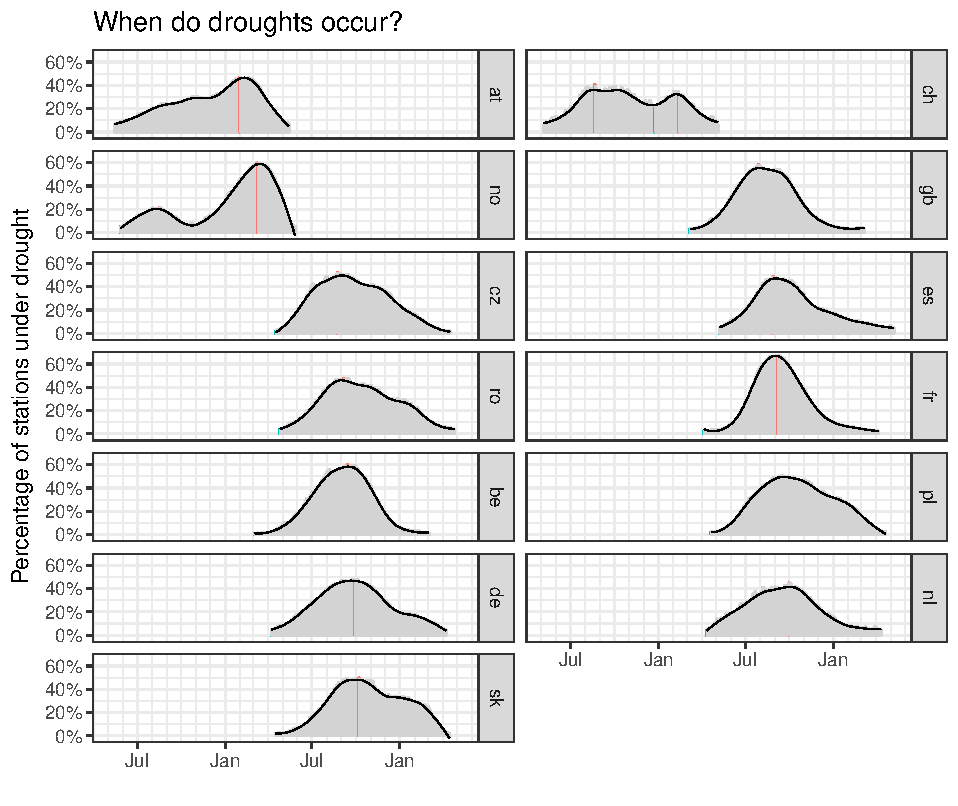
\includegraphics[height=\textheight]{./fig/hyear_start.pdf}   
\end{frame}


\end{document}